% Chapter 3
\chapter{Graphs that are levelable} % Chapter title

\label{ch:levelable-results} % For referencing the chapter elsewhere, use \autoref{ch:chaptername}

In this chapter we identify classes of graphs that are levelable. We also show that certain operations on graphs preserve levelability.

\section{Well-covered graphs}

The concept of a vertex cover was first introduced by \cite{Plummer1970}, is closely related to the maximal independent sets of a graph. Here we will connect the notions of minimal vertex covers to the facets of the independence complex, and use \autoref{thm:pure} to show that all well-covered graphs are levelable. Let us first define well-coveredness:

\begin{definition}
Let $G$ be a graph on $n$ vertices. A \textbf{vertex cover} of $G$ is a subset of vertices of $G$ such that every edge in $G$ is incident to some vertex in the vertex cover. A \textbf{minimal vertex cover} is a a vertex cover that fails to be a vertex cover if any of its vertices are removed. A graph $G$ is \textbf{well-covered} if every minimal vertex cover is of the same size. 
\end{definition}

We now relate the ideas of minimal vertex covers and maximal independent sets.

\begin{lemma}
A subset of vertices $X \subset V(G)$ is a minimal vertex cover if and only if $V(G) \setminus X$ is a maximal independent set. 
\end{lemma}
\begin{proof}
Let $G$ be a graph, and let $X \subset V(G)$ be a minimal vertex cover of $G$. Let $v, w \in V(G) \setminus X$. Then $\br{v, w} \not \in E(G)$, otherwise either $v$ or $w$ would be in $X$ in order for $X$ to be a vertex cover. So the complement of a vertex cover is an independent set. Furthermore, $V(G) \setminus X$ is maximal. If $(V(G) \setminus X)\cup\br{v'}$ (where $v' \in X$) was an independent set, then $(V(G) \setminus X) \cup {v'})^C = X \setminus \br{v'}$ would be a vertex cover. But then $X$ is not a minimal vertex cover. 
\end{proof}

Finally, we will apply \autoref{thm:pure} to show well-covered graphs are levelable.

\begin{theorem}
All well-covered graphs are levelable.
\end{theorem}
\begin{proof}
Let $G$ be a graph and $X_1, \dots, X_t$ denote the minimal vertex covers of $G$. Let  $F_i = V(G) \setminus X_i$ for $i = 1, \dots, t$. Then $F_1, \dots, F_t$ are maximal independent sets of $G$. If $G$ is well-covered, then $|X_1| =  \cdots = |X_t| = \lambda$. But then for any $i$, we have that $|F_i| = |V(G)| - |X_i| = |V(G)| - \lambda$. So $|F_1| = \cdots = |F_t| = |V(G)| - \lambda$. That is, all facets of the independence complex are the same size. Then, by \autoref{thm:pure}, $G$ is levelable.
\end{proof}

\section{Caterpillar graphs that are levelable} \label{sec:caterpillar}

We now discuss a particular type of graph called caterpillar graphs.

\begin{definition}
A graph $G$ is called a \textbf{caterpillar graph} if all the vertices of $G$ are all within distance 1 of a central path, and $G$ is cycle-free. Vertices that are not on the central path are called \textbf{legs} of $G$.
\end{definition}
\begin{figure}[bth]
    \myfloatalign
    {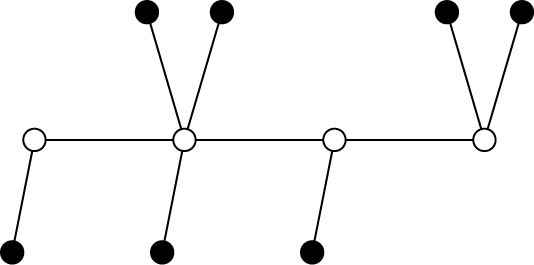
\includegraphics[width=.42\linewidth]{figures/caterpillar.png}} 
    \caption{An example of a caterpillar graph. Vertices on the central path are shown in white, and legs are shown in black.}
\end{figure}

In general, it is not true that all caterpillar graphs are levelable. As a counterexample, a caterpillar with no legs and a central path of length 5 is simply the path on 5 vertices, which is not levelable. However, the following theorem gives us a sufficient condition for levelability on caterpillar graphs.

\begin{theorem} \label{thm:caterpillar}
Let $G$ be a caterpillar graph. If every vertex on the central path of $G$ has at least one leg (except perhaps the endpoints of the path), then $G$ is levelable.
\end{theorem}

\begin{proof}
Suppose $G$ is caterpillar graph on $N$ vertices. Denote vertices on the central path by $p_1, \dots, p_n$. Let $L_i$ denote the set of legs that are adjacent to $p_i$. We can assume, without loss of generality, that $L_i \neq \emptyset$ for all $i$. If any of the endpoints $p_1$ or $p_n$ does not have a leg, then we can relabel the vertices such that $p_1$ as a leg of $p_2$ and/or $p_{n}$ as a leg of $p_{n-1}$. Let us then set a solution to the system in \autoref{thm:level-condition} as follows:
\begin{enumerate}
\item for any leg vertex $v_\alpha \in L_1 \cup \dots \cup L_n$, set $v_\alpha = 2$, and
\item for a vertex $p_i$ on the central path, set $p_i =  |L_i| + 1 $.
\end{enumerate}
Note that each $L_i$ is an independent set, since every leg in $L_i$ is adjacent to $p_i$, and if two legs in $L_i$ were adjacent this would create a cycle. Then, if $\ang{F_1, \dots, F_t}$ denotes the maximal independent sets of $G$, then each $F$ must satisfy either $p_i \in F$ or $L_i \subset F$ for each $i = 1, \dots, n$. Consider any two facets $F_a$ and $F_b$. Let $X = \br{i \; | \; i = 1, \dots, n}$, $A = \br{i \; | \; L_i \in F_a}$, and $B = \br{i \; | \; L_i \in F_b}$. The equation
\begin{equation*}
\begin{aligned}
S(F_a) - S(F_b) = |F_a| - |F_b|.
\end{aligned}
\end{equation*}
can therefore be written 
\begin{equation*}
\begin{aligned}
\left[S\left( \bigcup_{i \in A} L_i \right) + 
S\left( \bigcup_{i \in X \setminus A} \br{p_i} \right) \right] - 
\left[S\left( \bigcup_{i \in B} L_i \right) +
S\left( \bigcup_{i \in X \setminus B} \br{p_i} \right) \right] \\= \left|\bigcup_{i \in A} L_i \right| + |X \setminus A| - \left|\bigcup_{i \in B} L_i \right| -|X \setminus B|.
\end{aligned}
\end{equation*}
Substituting our proposed solution yields
\begin{equation*}
\begin{aligned}
2 \sum_{i \in A} |L_i| + \sum_{i \in X\setminus A} (|L_i| + 1)  - 2 \sum_{i \in B} |L_i| - \sum_{i \in X \setminus B} (|L_i| + 1) \\
= \sum_{i \in A} |L_i| + |X \setminus A| - \sum_{i \in B} |L_i| - |X \setminus B|,
\end{aligned}
\end{equation*}
which, by cancelling sums on each side, can be simplified to 
\begin{equation*}
\begin{aligned}
 \sum_{i \in A} |L_i|  +  \sum_{i \in X\setminus A} (|L_i| + 1) - \sum_{i \in B} |L_i| -  \sum_{i \in X \setminus B} (|L_i| + 1) 
= |X \setminus A| - |X \setminus B|.
\end{aligned}
\end{equation*}
Expanding constants in the sums yields
\begin{equation*}
\begin{aligned}
 \sum_{i \in A} |L_i|  +  \sum_{i \in X\setminus A} |L_i|  + |X \setminus A| - \sum_{i \in B} |L_i| -  \sum_{i \in X \setminus B} |L_i| - |X \setminus B|
= |X \setminus A| - |X \setminus B|,
\end{aligned}
\end{equation*}
i.e.,
\begin{equation*}
\begin{aligned}
 \sum_{i \in A} |L_i|  +  \sum_{i \in X\setminus A} |L_i|  - \sum_{i \in B} |L_i| -  \sum_{i \in X \setminus B} |L_i| = 0,
\end{aligned}
\end{equation*}
or equivalently
\begin{equation*}
\begin{aligned}
 \smashoperator{ \sum_{i \in A \cup (X \setminus A)}} |L_i|  \; \; - \; \; \smashoperator{\sum_{i \in B \cup (X \setminus B)}} |L_i|= 0,
\end{aligned}
\end{equation*}
since any set and its complement are disjoint. Since $F_1, \dots, F_t$ are all the facets of $G$, we have found a solution that satisfies $S(F_k) - S(F_{k+1}) = |F_k| - |F_{k+1}|$ for all $i$, and by \autoref{thm:level-condition} $G$ is levelable.
\end{proof}

\begin{example} \label{ex:levelable-caterpillar}(Levelable Caterpillar Graph) 
Let $G$ be a graph with:
\begin{itemize}
\item vertex set $V(G) = \br{p_1, p_2, p_3, q_1, \dots, q_6}$, and 
\item edge set $E(G) = \br{
\br{p_1, p_2},
\br{p_2, p_3},
\br{p_1, q_i \, | \, i = 1, 2},
\br{p_2, q_3},
\br{p_3, q_i \, | \, i = 4, 5, 6}
}.$
\end{itemize}
For a picture, see \autoref{fig:caterpillar-ex}. 

Here $p_1, p_2, p_3$ form the central path, and their corresponding leg vertices are $L_1 = \br{q_1, q_2}$, $L_2 = \br{q_3}$, and $L_3 = \br{q_4, q_5, q_6}$. As per \autoref{thm:caterpillar}, we will show that we can construct a levelable solution by setting
\begin{itemize}
\item $q_1 = \cdots = q_6 = 2$, 
\item $p_1 = |L_1| + 1 = 3$,
\item $p_2 = |L_2| + 1 = 2$, and
\item $p_3 = |L_3| + 1 = 4$.
\end{itemize}
Now, the maximal independent sets of $G$ are
\begin{itemize}
\item $F_1 = \br{p_1} \cup L_2 \cup \br{p_3} = \br{p_1, p_3, q_2}$,
\item $F_2 = \br{p_1} \cup L_2 \cup L_3 = \br{p_1, q_3, q_4, q_5, q_6}$,
\item $F_3 = L_1 \cup \br{p_2} \cup L_3 = \br{p_2, q_1, q_2, q_4, q_5, q_6}$,
\item $F_4 = L_1 \cup L_2 \cup \br{p_3} = \br{q_1, q_2, q_3, p_3}$
\item $F_5 = L_1 \cup L_2 \cup L_3 = \br{q_1, q_2, q_3, q_4, q_5, q_6}$,
\end{itemize}
We therefore have 4 equations in our system. The first is given by $S(F_1) - S(F_2) = |F_1| - |F_2|$, where 
\begin{itemize}
\item $S(F_1) = S(\br{p_1, p_3}) + S(L_1) = (3 + 4) + (2) = 9$,
\item $S(F_2) = S(\br{p_1}) + S(L_2 \cup L_3) =  (3) + (4 \cdot 2) = 11$,
\item $|F_1| = 3$, and
\item $|F_2| = 5$. 
\end{itemize} 
Then the first equation is satisfied, since
$$
S(F_1) - S(F_2) = 9 - 11 = -2 = 3 - 5 = |F_1| - |F_2|.
$$
The second equation is given by $S(F_2) - S(F_3) = |F_2| - |F_3|$, where
\begin{itemize}
\item $S(F_3) = S(\br{p_2}) + S(L_1 \cup L_3) = (2) + (5 \cdot 2) = 12$, and
\item $|F_3| = 6$.
\end{itemize} 
The second equation is satisfied since
$$
S(F_2) - S(F_3) = 11 - 12 = -1 = 5 - 6 = |F_2| - |F_3|.
$$
The third equation is given by $S(F_3) - S(F_4) = |F_3| - |F_4|$ where
\begin{itemize}
\item $S(F_3) = S(L_1 \cup L_2) + S(\br{p_3}) = (3 \cdot 2) + (3+1) = 10$, and
\item $|F_4| = 4$.
The third equation is satisfied, since
$$
S(F_3) - S(F_4) = 12 - 10 = 2 = 6 - 4 = |F_3| - |F_4|.
$$
\end{itemize}
The fourth and final equation is given by $S(F_4) - S(F_5) = |F_4| - |F_5|$ where
\begin{itemize}
\item $S(F_5) = S(L_1 \cup L_2 \cup L_3) = (6 \cdot 2) = 12$ and
\item $|F_5| = 6$.
\end{itemize}
This equation is also satisfied since 
$$
S(F_4) - S(F_5) = 10 - 12 = -2 = 4 - 6 = |F_4| - |F_5|,
$$
and so we have found a valid solution and $G$ is therefore levelable.
\end{example}
\begin{figure}[bth] 
    \myfloatalign
    \vspace{0.25cm}
    {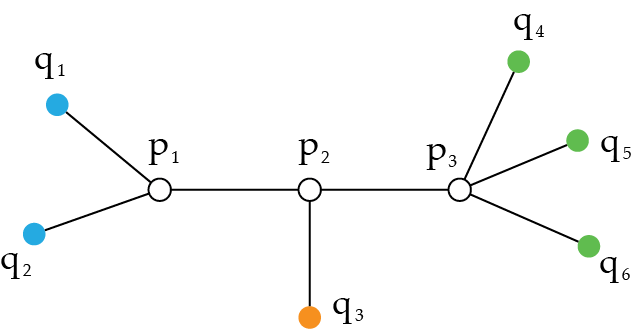
\includegraphics[width=.45\linewidth]{figures/caterpillar-ex.png}} 
    \caption{The levelable caterpillar graph described in \autoref{ex:levelable-caterpillar}. The central path is shown in white, while $L_1$, $L_2$, and $L_3$ are shown in blue, orange, and green respectively.} \label{fig:caterpillar-ex}
\end{figure}

It is interesting to note that every caterpillar graph on 4 or fewer vertices must satisfy the condition in \autoref{thm:caterpillar}. For example, the path graph on 4 vertices can be thought of as a caterpillar on a central path of 2 vertices, each adjacent to one leg vertex. However, any path graph on $n \geq 5$ vertices does not satisfy the condition, and none of these are levelable. This observation leads us to the converse statement of \autoref{thm:caterpillar}:

\begin{question}
Let $G$ be a caterpillar graph on 5 or greater vertices. If $G$ is levelable, does every vertex on the central path has at least one leg?
\end{question}

We also observe that this hypothesis is consistent with our computer search. That is, all levelable caterpillars on $n \leq 10$ vertices satisfy the condition in \autoref{thm:caterpillar}, and every non-levelable caterpillar has at least one vertex on the central path that does not have a leg.

\section{Complete multipartite graphs}

In this section we show that all complete multipartite graphs are levelable using a result from \cite{VanTuyl2010}. First, let us state the result.

\begin{theorem}[Theorem 12(iii) from \cite{VanTuyl2010}] \label{thm:pairwise-disjoint}
Any simplicial complex $\Delta$ with pairwise disjoint facets is levelable.
\end{theorem}

This result can be related to independence complexes on complete multipartite graphs, which are defined as follows:

\begin{definition} \label{def:complete-multipartite}
Let $G$ be graph on $n_1 + \dots + n_k$ vertices. Then $G$ is a \textbf{complete multipartite} graph or more specifically, a \textbf{complete $k$-partite graph} if its vertex set $V(G)$ can be expressed as $k$ disjoint sets $V_1$, \dots, $V_k$ such that the edge set $E(G)$ can be written 
$$
E(G) = \br{ \br{v, w} \, | \, v \in V_i, \, w \in V_j, \, i \neq j }.
$$
\end{definition}

\begin{theorem} \label{thm:complete-multipartite}
All complete multipartite graphs are levelable.
\end{theorem}

\begin{proof} 
If $G$ is a complete multipartite graph, then its maximal independent sets are pairwise disjoint. We will prove this by showing that the $k$ maximal independent sets of $G$ are exactly the $k$ disjoint sets $V_1, \dots, V_k$ as described in \autoref{def:complete-multipartite}. Notice first that the edge set does not contain any edges with endpoints within the same $V_i$. Thus each $V_i$ is an independent set. Then, notice that every vertex $v \in V_i$ is adjacent to all vertices $w \in V(G) \setminus V_i$. Thus $V_i$ is a maximal independent set. By construction $V_1, \dots, V_k$ are pairwise disjoint. Therefore by \autoref{thm:pairwise-disjoint}, all complete multipartite graphs are levelable.
\end{proof}

We can apply this result to star graphs, which were observed to be levelable in \autoref{subsec:star}.

\begin{corollary}
All star graphs are levelable.
\end{corollary}

\begin{proof}
The star graph on $n+1$ vertices is a complete 2-partite (``bipartite") graph. If we label the vertices as in \autoref{def:star}, then $V_1 = \br{v_0}$  and $V_2 = \br{v_1, \dots, v_{n}}$ give two disjoint vertex subsets such that 

\begin{enumerate}
\item there are no edges between pairs of vertices where both vertices are from either $V_1$ and $V_2$, and
\item all vertices in $V_1$ are adjacent to all vertices in $V_2$, since $v_0$ is adjacent to the other $n$ vertices.
\end{enumerate}

Thus, the star graph is a complete bipartite, and levelable by \autoref{thm:complete-multipartite}.
\end{proof}

\begin{figure}[bth]
    \myfloatalign
    {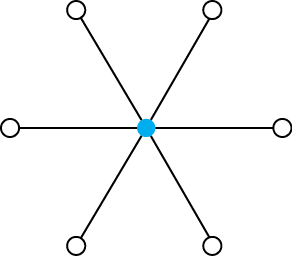
\includegraphics[width=.3\linewidth]{figures/star.png}} 
    \caption{The star on 7 vertices. The central vertex $v_0$ is shown in blue.}
\end{figure}



% --------------------------------------------------------------------------
% -------------------------------------------------------------------------

\section{Graph expansions}
We will now discuss operations on graphs that preserve the levelable property. Given a graph that is levelable, we can construct other levelable graphs by applying an "expansion" operation on the graph.

\begin{definition} \label{def:graph-expansion}
Let $G$ be a graph on $n$ vertices. A \textbf{graph expansion} $G'$ of $G$ is any graph where each vertex $v_i$ is replaced with a set of independent vertices $V_i = \br{v_{i, 1}, \cdots, v_{i, k_i}}$, and a vertex $v \in V_i$ is adjacent to a vertex in $w \in V_j$ if and only if $v_i$ and $v_j$ are adjacent in $G$. The sets $V_1, \dots, V_n$ that make up $V(G')$ are called \textbf{replica sets}, and a vertex $v \in V_i$ is called a \textbf{replica} of the \textbf{original vertex} $v_i$. Furthermore, we call $G'$ a \textbf{$k$-uniform expansion} if $|V_i| = k$ for $k = 1, \dots, n$. 
\end{definition}

An illustration of a graph expansion is given in \autoref{fig:expansion-ex}.

\begin{figure}[bth] 
    \myfloatalign
    \subfloat
    {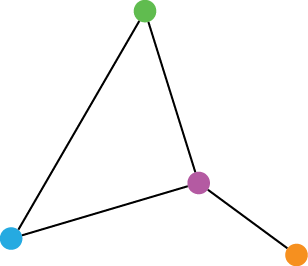
\includegraphics[width=.25\linewidth]{figures/expansion-before.png}} \\
    \subfloat
    {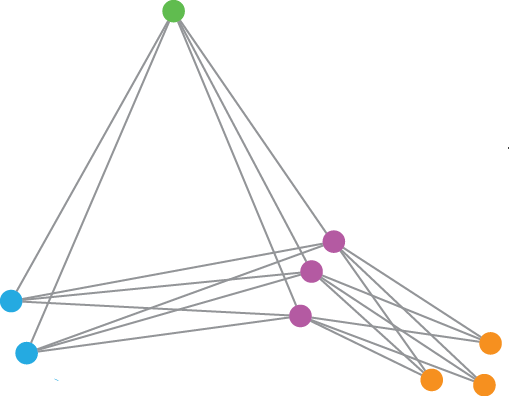
\includegraphics[width=.40\linewidth]{figures/expansion-nonuniform.png}} \\
    \subfloat
    {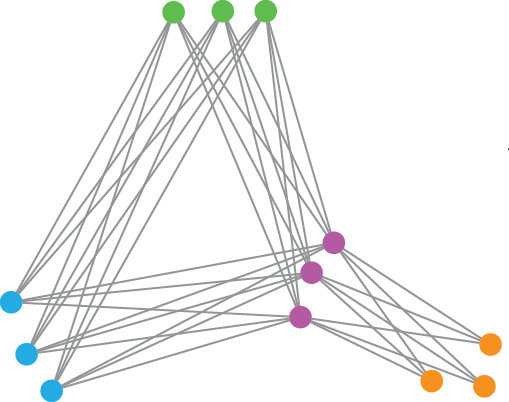
\includegraphics[width=.47\linewidth]{figures/expansion-uniform.png}} 
    \caption{A graph $G$ on 4 vertices (top); a non-uniform expansion of $G$ (middle); a 3-uniform expansion of $G$ (bottom). Replica sets are shown in the same colour as their original vertex.}\label{fig:expansion-ex}
\end{figure}

\begin{theorem} \label{thm:expansion}
Let $G$ be a levelable graph. Then any uniform expansion $G'$ of $G$ is levelable.
\end{theorem}
\begin{proof}
Since $G$ is levelable, let $(x_1, \dots, x_n)$ be a solution to \autoref{thm:level-condition}. Let $G'$ be a $k$-uniform expansion of $G$, and label the vertices $w_1, \dots, w_{nk}$ such that the first $k$ vertices correspond to $V_1$ in the expansion, the next $k$ vertices correspond to $V_2$, and so on. Then we claim that the $nk$-tuple $$(x_{1,1}, \dots, x_{1, k}, x_{2, 1}, \dots, x_{2, k}, \dots,x_{n, 1}, \dots, x_{n, k})$$ where $x_{i, j} = x_i$ is a solution to the the system in \autoref{thm:level-condition} for $G'$. 
First, we will show that the maximal independent sets of $G'$ are of the form 
\begin{equation*} \label{eq:expansion-union}
F' = \bigcup_{\br{\alpha: \, v_\alpha \in F}}  V_\alpha 
\end{equation*}
where $F$ is a maximal independent set in $G$. First, we note that for any maximal independent set $F'$ of $G'$, if some replica vertex is in $F'$, then all other vertices in its replica set will also be in $F'$. So $F'$ must be a union of replica sets.

It then follows from the construction of the expansion that replica sets are adjacent if and only if their corresponding original vertex was adjacent. That is,
$$
V_i \cup V_j \, \textrm{is an independent set} \Leftrightarrow N(V_i) \cap V_j = \emptyset \Leftrightarrow \br{v_i, v_j} \not \in E(G).
$$
We can then conclude that the maximal independent sets of $G'$ arise precisely out of corresponding maximal independent sets of $G$. 

Now, if $F_1, \dots, F_t$ are the maximal independent sets of $G$, then $F_1' \dots, F_t'$ are the maximal independent sets of $G'$. Consider any of the $t-1$ equations in \autoref{thm:level-condition}, each of the form
\begin{equation*}
\begin{aligned}
S(F_i') - S(F_{i+1}') = |F_i'| - |F_{i+1}'|.
\end{aligned}
\end{equation*}
Note that each facet $F'$ has $k$ times as many vertices as $F$, and so $|F'| = k |F|$. In addition, by substituting our proposed solution, for any replica set $V_i$, $S(V_i) = k v_i$. Since each $F'$ is made of a union of replica sets and replica sets are pairwise disjoint, $S(F') = k S(F)$. Therefore, we can write the above equation as
\begin{equation*}
\begin{aligned}
kS(F_i) - kS(F_{i+1}) = k|F_i| - k|F_{i+1}|,
\end{aligned}
\end{equation*}
to which there is a solution when $G$ is levelable.
\end{proof}

\section{Adding vertices} \label{sec:adding-vertices-levelable}

Here we will show that adding vertices (up to a certain number) adjacent to all existing vertices of the graph preserves the levelable condition.

\begin{theorem} \label{thm:vertex-add}
Let $G$ be a levelable graph and let $F_1, \dots, F_t$ denote the facets of $\ind(G)$. Define $G'$ to be the graph with vertex set $V(G') = V(G) \cup \br{w_1, \dots, w_m}$ and edge set $E(G') = E(G) \cup \br{\br{v_i, w_j} \; | \; v_i \in V(G), j = 1, \dots, m}$, where $m \leq |F_t|$. Then $G'$ is levelable.
\end{theorem}

\begin{proof}
If $F_1, \dots, F_t$ are the facets of $\ind(G)$, Then $F_1, \dots, F_t, \br{w_1, \dots, w_m}$ are the facets of $\ind(G')$, since each $w_i$ is adjacent to every vertex in $V(G)$ but independent of all $w_j$ for $i \neq j$. Since $G$ is levelable, there exists some solution $(a_1, \dots, a_n)$ to the system in \autoref{thm:level-condition} for $G$.

If we set $b_1 = \cdots b_{m-1} = 2$ and $b_m = S(F_t) - m + 2 - |F_t|$, then $(a_1, \dots, a_n, \allowbreak b_1, \dots, b_m)$ is a solution to the system of $t$ equations for $G'$, where $b_i$ corresponds to $w_i$. 

Notice first that the first $t-1$ equations $S(F_i) - S(F_{i+1})  = |F_i| - |F_{i+1}|$ for $t = 1, \dots, t-1$ are unchanged from $G$, and are independent of $w_1, \dots, w_m$. Then, the $t^{\textrm{th}}$ equation is 
$$
S(F_t) - b_1 - \cdots - b_m = |F_t| - m.
$$
If we take $b_1 = \cdots = b_{m-1} = 2$ and $b_m = S(F_t) - m + 2 - |F_t| \geq 2$, then
\begin{equation*}
\begin{aligned}
S(F_t) - b_1 - \cdots - b_m &= S(F_t) - 2(m-1) - S(F_t) + m - 2 + |F_t| \\ &= -2m + 2  + m  - 2 +| F_t| \\&= -m + |F_t|.
\end{aligned}
\end{equation*}
as required. Furthermore $b_m \geq 2$, since, when $|F_t| \geq m$ we have
$$
b_m = S(F_t) - m + 2 - |F_t| \geq S(F_t) - |F_t| + 2 - |F_t| \geq 2|F_t| - |F_t| + 2 - |F_t| = 2.
$$
Thus a valid solution exists and $G'$ is levelable.
\end{proof}

\begin{example} \label{ex:star-add}
Let $G$ be the star on 4 vertices labelled $v_1, \dots, v_4$ where $v_1$ is the central vertex. Since $G$ is a graph on only 4 vertices, by \autoref{thm:small} it is levelable. The two maximal independent sets of $G$ are given by 
$F_1 = \br{v_1}$ and 
$F_2 = \br{v_2, v_3, v_4}$.
Now, let $G'$ be the graph with vertex set $V(G') = V(G) \cup \br{w_1, w_2}$ and edge set $E(G) = \br{ \br{v_i, w_j} \; | \; i = 1, \dots, 4; \, j = 1, \dots, 2}$. Since $G$ is levelable, there exists a solution to the system in \autoref{thm:level-condition}. In particular, a solution is given by $(v_1, v_2, v_3, v_4) = (4, 2, 2, 2)$:
$$
S(F_1) - S(F_2) = 4 - 3(2) = -2 = 1 - 3 = |F_1| - |F_2|.
$$
The corresponding system for $G'$ has one additional facet $F_3 = \br{w_1, w_2}$ and a solution given by $(v_1, v_2, v_3, v_4, w_1, w_2) = (4, 2, 2, 2, 2, 3)$, where the value of $w_3$ arises from $S(F_2) - m + 2 - |F_2| = 6 - 2 + 2 - 3 = 3$ as per \autoref{thm:vertex-add}. Indeed, this is a solution since
$$
S(F_2) - S(F_3) = 3(2) - 2 - 3 = 1 = 3 - 2 = |F_2| - |F_3|,
$$
and $G$ is levelable.

\begin{figure}[h]
    \myfloatalign
    \subfloat
    {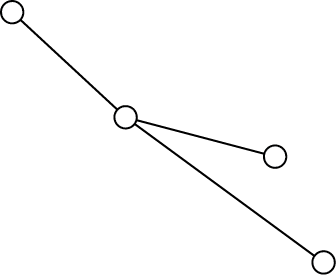
\includegraphics[width=.26\linewidth]{figures/4-star-before.png}} \qquad
    \subfloat
    {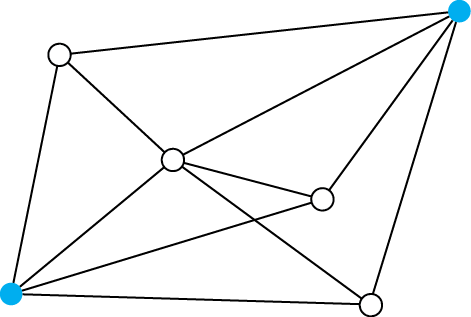
\includegraphics[width=.37\linewidth]{figures/4-star-addition.png}}
    \caption{The star on 4 vertices (left) and the graph $G'$ (right) constructed in \autoref{ex:star-add} by adding two additional vertices shown in blue.}
\end{figure}

\end{example}


\chapter{Graphs that are not levelable}

\label{ch:non-levelable-results}

In this chapter we discuss conditions that preclude levelability. In particular, in \autoref{sec:large-cycles} we show that large cycles are not levelable, and in \autoref{sec:criteria} we introduce a criterion on the independent sets of a graph that allows us to conclude that certain trees, including all paths on large numbers of vertices, are not levelable. Finally, in \autoref{sec:adjoinment} we show that attaching a non-levelable graph in a certain way will always result in a non-levelable graph.

\section{Large cycles} \label{sec:large-cycles}

In \autoref{subsec:cycles-wheels}, we noted that cycles were observed to fail to be levelable. We begin this chapter by proving this fact for cycles of arbitrary size $n \geq 8.$

\begin{theorem}\label{thm:cycles}
Let $G$ be the cycle graph on $n$ vertices, where $n \geq 8$. Then $G$ is not levelable.
\end{theorem}
\begin{proof}
Label the $n$ vertices clockwise in increasing order $v_1, \dots, v_n$. Then we have that the edge set is $E(G)= \br{ \br{v_i, v_{i+1}} \, | \,i = 1, \dots, n-1} \cup \br{\br{v_1, v_n}}$. Suppose, for a contradiction that $(x_1, \dots, x_n)$ is a solution that satisfies \autoref{thm:level-condition}.

First, we note that a maximal independent set $F$ of $G$ is a selection of vertices from the cycle such that any vertex in $F$ is distance 2 or  3 from another vertex in $F$ , but not more. These are independent sets, since we have chosen vertices that are not adjacent in the cycle. Furthermore, these are maximal since any smaller selection would have a gap of 3 or more vertices in the cycle. We could then properly include such a selection in a larger independent set by taking a middle vertex in the gap of 3 or more vertices. 

\noindent
\underline{Case}: $n$ is even.  
Take $F_1$ to be the set of even-numbered vertices $F_1 = \br{v_2, v_4, \dots, v_n}$, and take $F_2$ to be the set of all even numbered vertices up to $v_{n-4}$ inclusive, and $v_{n-1}$. So $F_2 = \br{v_2, v_4, \dots, v_{n-4}, v_{n-1}}$. Then  $S(F_1) - S(F_2) = |F_1| - |F_2|$, i.e.,
\begin{equation*}
\begin{aligned}
(x_2 + x_4 + \cdots + x_n) - (x_2, x_4, \dots, x_{n-4}, x_{n-1}) &= \frac{n}{2} - \left(\frac{n}{2} - 1\right) = 1,
\end{aligned}
\end{equation*}
which reduces to
\begin{equation}\label{eq:cycle-1}
\begin{aligned}
x_{n-2} + x_n - x_{n-1} &= 1.
\end{aligned}
\end{equation}
Take $F_3 = \br{v_2, v_4, \dots, v_{n-6}, v_{n-3}, v_{n-1}}$ and $F_4 = \br{v_2, v_4, \dots, v_{n-6}, v_{n-3}, v_n}$. Then $S(F_3) - S(F_4) = |F_3| - |F_4|$, i.e.,
\begin{equation*}
\begin{aligned}
(x_2, x_4, \dots, x_{n-6}, x_{n-3}, x_{n-1}) - (x_2, x_4, \dots, x_{n-6}, x_{n-3}, x_{n-1}) = 0
\end{aligned}
\end{equation*}
which reduces to
\begin{equation} \label{eq:cycle-2}
\begin{aligned}
x_{n-1} & = x_n.
\end{aligned}
\end{equation}
Combining the information from \eqref{eq:cycle-1} and \eqref{eq:cycle-2} we obtain $x_{n-2} + x_n - x_{n-1} = x_{n-2} + x_n - x_n = 1$ which gives a contradiction, since we require all $x_i \geq 2$. Thus $G$ is not levelable for even $n$.

\noindent
\underline{Case}: $n$ is odd. 
Take $F_1$ to be the even-labelled vertices $\br{v_2, \dots, v_{n-1}}$ and $F_2 = \br{v_1, v_3, v_6, v_8 \dots, v_{n-1}}$. Then $S(F_1) -S(F_2) = |F_1| - |F_2| = 0$, i.e.,
\begin{equation*}
\begin{aligned}
(x_2 + \dots + x_{n-1}) - (x_1 + x_3 + x_6 + x_8 + x_{n-1}) &= 0 
\end{aligned}
\end{equation*}
which reduces to
\begin{equation}\label{eq:odd1}
\begin{aligned} 
x_2 + x_4 &= x_1 + x_3.
\end{aligned}
\end{equation}
Then take $F_3 = \br{v_1, v_4, v_6, v_8 \dots, v_{n-1}}$, and $S(F_2) -S(F_3) = |F_2| - |F_3|$ gives
$$
(x_1 + x_3 + x_6 + x_8 + \cdots + x_{n-1}) - (x_1 + x_4 + x_6 + x_8 + \cdots + x_{n-1}) = 0
$$
which reduces to
\begin{equation}
\begin{aligned}
\label{eq:odd2}
x_3 &= x_4.
\end{aligned}
\end{equation}
Combining the result from \eqref{eq:odd1} and \eqref{eq:odd2} gives $x_1 = x_2$. Now, take $F_4 = \br{v_2, v_4, v_6, \allowbreak \dots,  v_{n-5}, v_{n-2}, v_n}$. Since $S(F_3) -S(F_4) = |F_3| - |F_4| = 0$, we have that
\begin{equation*}
\begin{aligned}
(x_1 + x_4 + x_6 + x_8 + \cdots + &x_{n-3} + x_{n-1}) \\ &- (x_2 + x_4 + x_6 + \cdots+ x_{n-5} + x_{n-2}+ x_n) = 0, 
\end{aligned}
\end{equation*}
i.e.,
\begin{equation}
\begin{aligned}\label{odd3}
x_{n-3} + x_{n-1} &= x_{n-2} + x_n.
\end{aligned}
\end{equation}
Then take $F_5 =\br{ v_2, v_4, v_6, \dots, v_{n-5}, v_{n-3}, v_n}$. Since $S(F_4) -S(F_5) = |F_4| - |F_5| = 0$,
\begin{equation*}
\begin{aligned}
(x_2+ x_4+ x_6 + \cdots + x_{n-5} + &x_{n-2}+ x_n)  \\ &- (x_2+ x_4+ x_6 + \cdots + x_{n-5} + x_{n-3}+ x_n) = 0, 
\end{aligned}
\end{equation*}
which reduces to
\begin{equation} \label{odd4}
x_{n-2} = x_{n-3}.
\end{equation}
Combining the equalities from \eqref{odd3} and \eqref{odd4} yields $x_{n-1} = x_n$. Now, take $F_6 = \br{v_1, v_4, v_6, \dots, v_{n-5}, v_{n-2}}$. Then $S(F_5) - S(F_6) = |F_5| - |F_6|$ gives
\begin{equation*}
\begin{aligned}
\label{odd5}
(x_2+ x_4+ x_6 + \cdots + x_{n-5} + &x_{n-3}+ x_n) \\ &- (x_1 + x_4 + x_6 + \cdots + x_{n-5} + x_{n-2}) = 1,
\end{aligned}
\end{equation*}
and cancelling the common terms yields
\begin{equation*}
\begin{aligned}
(x_2+  x_{n-3}+ x_n) - (x_1 + x_{n-2}) &= 1. \\
\end{aligned}
\end{equation*}
But since $x_{n-3} = x_{n-2}$ and $x_2 = x_1$, we have that $x_n = 1$, which again, gives a contradiction since we require that any $x_i \geq 2$. So $G$ is also not levelable if $n$ is odd.
\end{proof}

\section{Criteria on vertex partitions} \label{sec:criteria}

In \autoref{sec:smallest}, we showed that the path on 5 vertices is not levelable. Here, we give a generalization of that result using a similar proof. Using this result, we rule out certain classes of tree graphs in \autoref{cor:balanced-trees}, which also lets us conclude that long paths are not levelable in \autoref{cor:long-paths}.

\begin{theorem} \label{thm:graph-partitions}
Let $G$ be a graph on $n$ vertices. If the vertex set of $G$, $V(G)$ has a partition $V(G) = V_1 \cup  \cdots \cup  V_5 \cup W$, and $Y \subset W$ such that 
\begin{equation} \label{eq:graph-partitions}
\begin{aligned}
F_1 &= V_1 \cup V_3 \cup V_5 \cup Y,\\
F_2 &= V_2 \cup V_4 \cup Y,\\
F_3 &= V_2 \cup V_5 \cup Y, \textrm{ and }\\
F_4 &= V_1 \cup V_4 \cup Y
\end{aligned}
\end{equation}
are maximal independent sets of $G$, then $G$ is not levelable.
\end{theorem}
\begin{proof}
Assume that $G$ is levelable. Then there exists some valid solution to the system in \autoref{thm:level-condition}. The first equation is given by
\begin{equation*}
\begin{aligned}
S(F_1) - S(F_2) = |F_1| - |F_2|.
\end{aligned}
\end{equation*}
Since $V_i$ and $V_j$ are disjoint for any $i \neq j$, this equation can be written as
\begin{equation*}
\begin{aligned}
S(V_1) + S(V_3) + S(V_5) + S(Y) - S(V_2) - S(V_4) - S(Y) \\
= |V_1| + |V_3| + |V_5| + |Y| - |V_2| - |V_4| -|Y|.
\end{aligned}
\end{equation*}
i.e., 
\begin{equation} \label{eq:5part1}
\begin{aligned}
S(V_1) + S(V_3) + S(V_5) - S(V_2) - S(V_4) = |V_1| + |V_3| + |V_5| - |V_2| - |V_4|.
\end{aligned}
\end{equation}
The second equation $S(F_2) - S(F_3) = |F_2| - |F_3|$ can similarly be written as
$$
S(V_2) + S(V_4)  +  S(Y) - S(V_1) - S(V_4) - S(Y) = |V_2| + |V_4| +|Y| - |V_1| - |V_4| - |Y|.
$$
Cancelling terms yields
\begin{equation} \label{eq:5part2}
\begin{aligned}
S(V_2) - S(V_1) = |V_2| - |V_1| .
\end{aligned}
\end{equation}
The final equation $S(F_3) - S(F_4) = |F_3| - |F_4|$ can be written as
\begin{equation*} 
\begin{aligned}
S(V_1) + S(V_4) + S(Y)- S(V_2) - S(V_5) - S(Y)= |V_1| + |V_4| + |Y|- |V_2| - |V_5| - |Y|,
\end{aligned}
\end{equation*}
that is,
\begin{equation} \label{eq:5part3}
\begin{aligned}
S(V_1) + S(V_4) - S(V_2) - S(V_5) = |V_1| + |V_4| -|V_2| - |V_5|.
\end{aligned}
\end{equation}
Applying the result from equation \eqref{eq:5part2} to \eqref{eq:5part3}, we obtain that
$$
S(V_1) + S(V_4) - S(V_2) - S(V_5) =  |V_4| - |V_5|  + S(V_1)  - S(V_2),
$$
i.e.,
\begin{equation} \label{eq:5part4}
\begin{aligned}
S(V_4) - S(V_5) &=  |V_4| - |V_5|.
\end{aligned}
\end{equation}
If we substitute the result from \eqref{eq:5part2} in the right-hand side of \eqref{eq:5part1}, we obtain
\begin{equation*}
\begin{aligned}
S(V_1) + S(V_3) + S(V_5) - S(V_2) - S(V_4) = S(V_1) + |V_3| + |V_5| - S(V_2) - |V_4|
\end{aligned}
\end{equation*}
Futhermore, applying the result from \eqref{eq:5part4} to the right-hand side of the above equation yields
$$
S(V_1) + S(V_3) + S(V_5) - S(V_2) - S(V_4) = S(V_1) + |V_3| + S(V_5) - S(V_2) + S(V_4).
$$
Cancelling common terms from both sides yields
$$
S(V_3) = |V_3|,
$$
but this means $G$ cannot be levelable. If a solution $(a_1, \dots, a_n)$ has $a_i \geq 2$ for all $i$, then it must be that $S(V_3) \geq 2 |V_3|$. 
\end{proof}
\noindent
We can apply the above result to trees to show that certain trees are not levelable. 

\begin{definition}
A graph $G$ is a \textbf{tree} if any two vertices $x$ and $y$ in $G$ can be connected by a unique simple path. That is, there is exactly one set of edges $\br{\br{x, v_1}, \dots, \br{v_n, y}}$ that connect $x$ and $y$. Furthermore, a \textbf{rooted tree} is a graph where one vertex has been designated the vertex. The \textbf{depth} of a vertex in a rooted tree is the length of the path from the vertex to the root. A vertex on a tree is called a \textbf{leaf} if it is connected only adjacent to one other vertex. The maximum depth of a leaf (or equivalently, the length of the longest path from a vertex to the root) is called the \textbf{height} of the tree. Lastly, a rooted tree is \textbf{balanced} if the depth of every leaf is the same.
\end{definition}

\begin{corollary} \label{cor:balanced-4-tree}
Balanced trees of height 4 are not levelable.
\end{corollary}
\begin{proof}
Let $G$ be a balanced tree of height 4. We can partition the vertices to satisfy \autoref{thm:graph-partitions} by taking $V_i$ to be the set of vertices at depth $i-1$ in the tree for $i = 1, \dots, 5$, and $W$ (and therefore $Y \subset W$) to be empty. Note that all vertices $V_i$ at a certain depth cannot be adjacent to each other, and so any maximal independent set $F$ is some union of the sets $V_1, \dots, V_4$. Furthermore, $V_i \subset F$ if and only if $V_{i-1} \cap F = V_{i+1} \cap F = \emptyset$. we can conclude that $F_1, \dots, F_4$ as described in \autoref{thm:graph-partitions} are indeed maximal independent sets of $G$, and therefore $G$ is not levelable.
\end{proof}

\begin{remark} Balanced trees of height 5 cannot easily be partitioned to satisfy \autoref{thm:graph-partitions}. The natural choice would be to let $V_i$ be all the vertices at depth $i-1$ for $i = 1, \dots, 5$  and let $W = Y$ be the vertices at depth 6. However, this does not satisfy \autoref{thm:graph-partitions} since $Y$ should be independent of all $V_i$ in order for the sets in \eqref{eq:graph-partitions} to be maximal independent sets, but $Y$ is adjacent to $V_5$. Therefore, to address this special case we require a different criterion. We discuss this problem further in \autoref{sec:other-criteria}. However, we can apply \autoref{thm:graph-partitions} to trees of height 6 or greater.
\end{remark}

\begin{corollary} \label{cor:balanced-trees}
Balanced trees of height 6 or greater are not levelable.
\end{corollary}

\begin{proof}
We will use the result from \autoref{thm:graph-partitions}. Let $G$ be a balanced tree of height $k$, where $k \geq$ 6. First, notice that for any $i$, the vertices of depth $i$ form an independent set. If any two vertices at depth $i$ were adjacent, this would be a path that connects the two in addition to the path that goes through the vertex. With this in mind, let $V_1 \subseteq V(G)$ contain only the root vertex. For $i = 2, \dots, k+1$, take $V_i$ to consist of all the vertices of depth $i-1$, and group together $W = V_6 \cup \cdots \cup V_{k+1}$. Then $V_1, \dots, V_5, W$ form a partition of $V(G)$. Moreover, if we take $Y \subseteq W$ to be a maximal independent set of $W$ such that $V_7 \subseteq Y$ (which is certainly possible since no vertices in $V_7$ are adjacent), then $F_1, \dots, F_4$ as defined in \autoref{thm:graph-partitions} are indeed maximal independent sets of $G$, and is therefore not levelable.
\end{proof}

\begin{figure}[bth]
    \myfloatalign
    {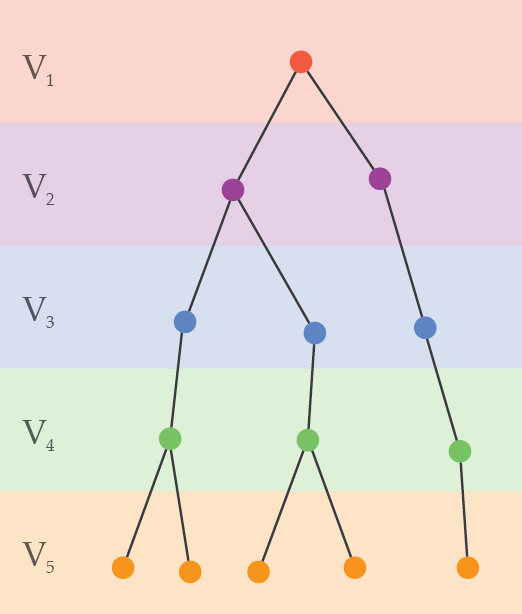
\includegraphics[width=.5\linewidth]{figures/5-tree-colour.png}} 
    \caption{An example of a balanced tree of height 4. Vertex partitions $V_1, \dots, V_5$ are coloured as described in \autoref{cor:balanced-4-tree}.}
\end{figure}

\noindent
Since paths are special cases of balanced trees, we can apply \autoref{cor:balanced-trees} to show that long paths are not levelable.

\begin{corollary} \label{cor:long-paths}
Paths on 7 or more vertices are not levelable.
\end{corollary}
\begin{proof}
Every path is also a balanced tree by taking an endpoint to be the root. There is then only one leaf (the other endpoint of the path), and therefore must be balanced. A path of length $n$ is hence a tree of height $n-1$ and by \autoref{cor:balanced-trees} is not levelable for $n \geq 7$.
\end{proof}

\section{Obstruction via graph adjoinment} \label{sec:adjoinment}

In this section we introduce a graph operation that ensures non-levelability by attaching a non-levelable graph.

\begin{definition}
If $A$ and $B$ are non-empty graphs, then $G$ is an \textbf{adjoinment} of $A$ and $B$ if $G = A\cup B \cup X$, where $X$ is a path with an endpoint in $A$ and the other in $B$. We call $X$ an \textbf{adjoining path} between $A$ and $B$. More generally, we call a graph $G$ a \textbf{$(p_1, \dots, p_k)$-adjoinment} of $A$ and $B$ if the vertex set of $G$ can be written 
\begin{equation*}
\begin{aligned}
V(G) = V(A)
\cup V(B) 
\cup V(X_1) \cup \cdots \cup V(X_k)
\end{aligned}
\end{equation*}
and the edge set 
\begin{equation*}
\begin{aligned}
E(G) =  E(A) \cup E(B) \cup E(X_1) \cup \cdots \cup E(X_k) 
\end{aligned}
\end{equation*}
where 
\begin{enumerate}
\item $V(X_i) = \br{v_{i, 1}, \dots, v_{i, p_i}}$,
\item $E(X_i) = \br{\br{v_{i, s}, v_{i, s+1}} \; | \; s = 1, \dots, p_{i} - 1 }$,
\item $V(A) \cap V(X_i) = \br{v_{i, 1}}$, and
\item $V(B) \cap V(X_i) = \br{v_{i, p_i}}$ 
\end{enumerate}
for $i = 1, \dots, k$. 
\end{definition}

\begin{figure}[!h]
    \myfloatalign
    {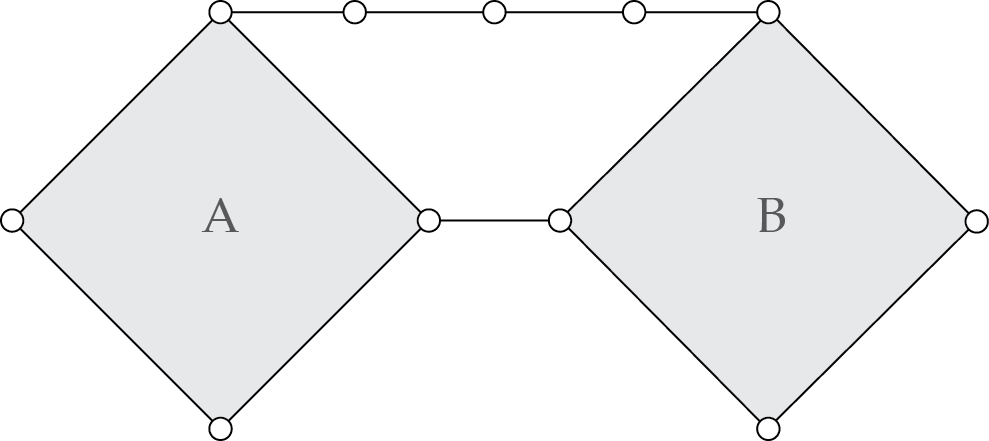
\includegraphics[width=.65\linewidth]{figures/adjoinment.png}} 
    \caption{A (5,2)-adjoinment of $A$ and $B$.}
\end{figure}

\begin{theorem}[Obstruction via adjoinment] \label{thm:adjoinment}
Let $A$ be a non-levelable graph on $V(A) = \br{v_1, \dots, v_n}$ and let $B$ be a graph on $V(B) = \br{w_1, \dots, w_m}$. Let $G$ be a $(p_1, \dots, p_k)$-adjoinment of $A$ and $B$ with $k \geq 1$ and $p_i \geq 4$ for all $i$. Then $G$ is also not levelable.
\end{theorem}

\begin{proof}
First, note that on every adjoinment path $X_i$, denote by $v_{i, 3}$ the vertex on the path that is distance 2 from $A$. Denote by $C_1, \dots, C_s$ the maximal independent sets of $A$, and let $D$ be a maximal independent set on $G \setminus A$ with $\br{v_{1,3}, \dots, v_{k,3}} \subseteq D$. To see why this is possible, note that since each path $X_i$ is on at least 4 vertices, every $v_{i,3}$ is adjacent only to $v_{i, 2}$ and $v_{i, 4}$ (and thus not adjacent to any $v_{j,3}$). 

It follows that for $i = 1, \dots, s$, $F_i = C_i \cup D$ is a maximal independent set of $G$. To check that these are independent sets, we need only check edges between $C_i$ and $D$. By construction of the adjoinment and choice of $D$, every vertex in $D$ is only connected to $A$ through some $v_{i, 3}$, and is therefore at least distance 2 from any vertex in $A$. So this is an independent set of $G$. To see that this is maximal, notice that we cannot add any vertex in $A$, since $C_i$ is maximal in $A$, and similarly we cannot add any vertex in $G \setminus A$, since $D$ is maximal in $G \setminus A$. 

Suppose then, that there exists some solution $(x_1, \dots, x_n, \dots, x_{N})$ to \autoref{thm:level-condition}, where $x_1, \dots, x_n$ correspond to the vertices in $A$. and the last $N-n$ correspond to the vertices in $G \setminus A$. The first $s-1$ equations of the system are
\begin{equation*}
S(F_i) - S(F_{i+1}) = |F_i| - |F_{i+1}|
\end{equation*}
for $i = 1, \dots, s-1$. However, given that $D$ is disjoint from each $C_i$, this is equivalent to
\begin{equation*}
S(C_i) + S(D) - S(C_{i+1}) - S(D) = |C_{i}| + |D| - |C_{i+1}| - |D|,
\end{equation*}
i.e.,
\begin{equation*}
S(C_i) - S(C_{i+1}) = |C_{i}|  - |C_{i+1}|
\end{equation*}
for $i = 1, \dots, s-1$. These equations depend only on vertices in $A$, and so if $(x_1, \dots, x_n, \dots, x_N)$ were a valid solution, then $(x_1, \dots, x_n)$ is a valid solution to these $s-1$ equations. However, this is exactly the system that needs to be satisfied in order for $A$ to be levelable, which gives a contradiction.
\end{proof}

Using the fact that the path on 5 vertices is not levelable, we can give an alternate proof for the non-levelability of cycles using \autoref{thm:adjoinment}.

\begin{corollary}
Cycle graphs on 10 or more vertices are not levelable.
\end{corollary}
\begin{proof}
Let $G = C(n)$ denote the cycle graph on $n \geq 10$ vertices. Then $G$ can expressed as a (4, 4)-adjoinment of $A$, the path graph on 5 vertices, and $B$, the path graph on $n-9$ vertices, where the adjoinment paths connect the endpoints of $A$ and $B$ to create a cycle. Since the path on 5 vertices is not levelable, applying \autoref{thm:adjoinment} tells us $G$ is not levelable.
\end{proof}

\begin{example} (The 10-cycle is not levelable). \label{ex:10-cycle}
Let $A$ denote the path on 5 vertices $\br{a_1, \dots, a_5}$ where $a_1$ and $a_5$ are the endpoints of the path, and $B$ denote the graph on 1 vertex $\br{b}$. Now, let $X_1$ be a path on 4 vertices $\br{v_{1, 1}, v_{1, 2}, v_{1,3}, v_{1,4}}$ 
where $v_{1,1}$ is a relabelling of $a_1$ and $v_{1,4}$ is a relabelling of $b$. Similarly, let $X_2$ be a path on 4 vertices $\br{v_{2, 1}, v_{2, 2}, v_{2, 3}, v_{2, 4}}$, where $v_{2, 1}$ is a relabelling of $a_5$ and $v_{2, 4}$ is a relabelling of $b$. Then $G = A\cup X_1 \cup X_2 \cup B$ is a (4, 4)-adjoinment of $A$ and $B$ (for an illustration, see \autoref{fig:10-cycle}). By \autoref{thm:adjoinment}, this graph is not levelable, since the path $A$ on 5 vertices is not levelable.

We verify this result with a specific application of the proof in \autoref{thm:adjoinment}. Notice that
\begin{equation}
\begin{aligned}
&C_1 = \br{a_1, a_3, a_5}, \\
&C_2 = \br{a_2, a_4}, \\
&C_3 = \br{a_2, a_5}, \textrm{ and }\\
&C_4 = \br{a_1, a_4}
\end{aligned}
\end{equation}
are maximal independent sets of $A$. Take $D = \br{v_{1,3}, v_{2,3}}$. Then $F_i = C_i \cup D$ is a maximal independent set of $G$ for $i = 1, \dots, 4$. Consider some potential solution $(a_1, \dots, a_5, b, v_{1,2}, v_{1,3}, v_{2, 2}, v_{2, 3})$. Notice that for any $S(F_i) - S(F_{i+1}) = |F_i| - |F_{i+1}|$, we can write this as 
\begin{equation}
\begin{aligned}
S(C_i) + S(D) - S(C_{i+1}) - S(D) = |C_i| + |D| - |C_{i+1}|- |D| 
\end{aligned}
\end{equation}
i.e., $S(C_i) - S(C_{i+1}) = |C_i| - |C_{i+1}|$. These equations depend only on vertices in $A$, and do not have a valid solution since the path on 5 vertices is not levelable.

\end{example}
\begin{figure}[bth]
    \myfloatalign
    \subfloat
    {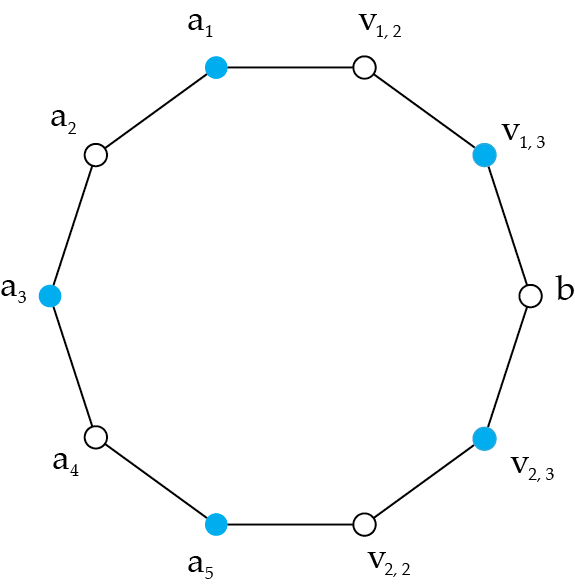
\includegraphics[width=.4\linewidth]{figures/cycle-adjoinment-1.png}} \qquad 
    \subfloat
    {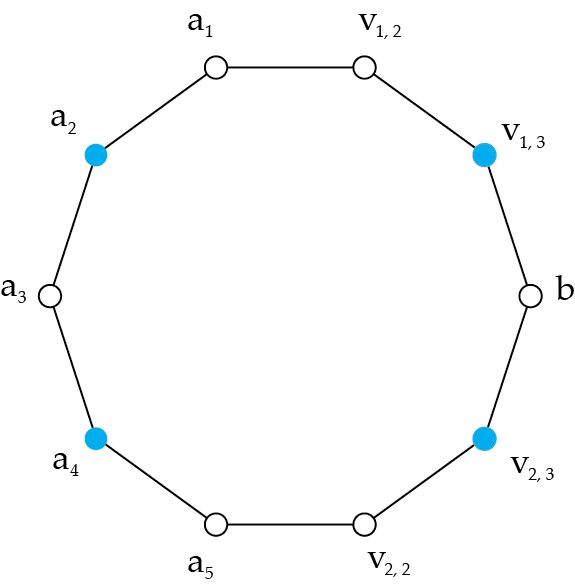
\includegraphics[width=.4\linewidth]{figures/cycle-adjoinment-2.png}} \\
    \subfloat
    {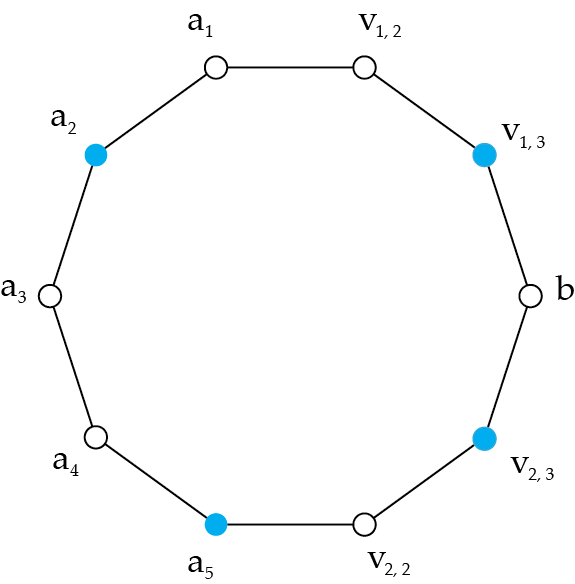
\includegraphics[width=.4\linewidth]{figures/cycle-adjoinment-3.png}} \qquad
    \subfloat
    {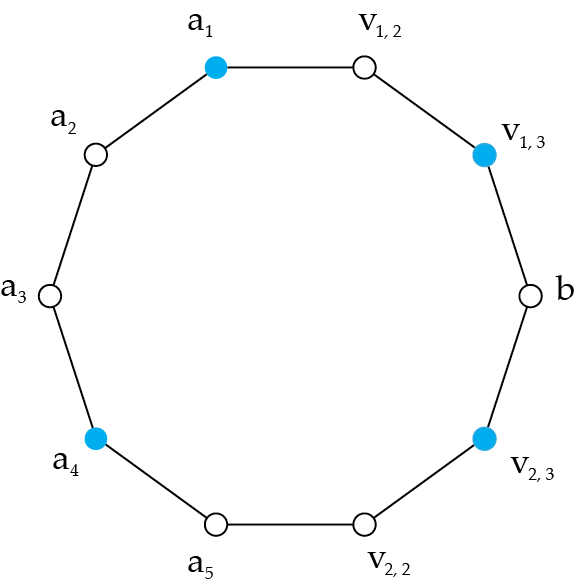
\includegraphics[width=.4\linewidth]{figures/cycle-adjoinment-4.png}}
    \caption{The cycle on 10 vertices labelled as a (4, 4)-adjoinment between the path on 5 vertices and the graph on 1 vertex as described in \autoref{ex:10-cycle}. Facets are shown in blue. Notice that the independent set $D = \br{v_{1, 3}, v_{2, 3}}$ is contained in every facet.} \label{fig:10-cycle}
\end{figure}

\section{Adding vertices} \label{sec:adding-vertices-non-levelable}
In \autoref{sec:adding-vertices-levelable}, we showed that adding vertices (up to some limit) preserves the levelability of a graph. In this section, we show a similar statement for non-levelable graphs. That is, adding vertices to a non-levelable graph will yield a non-levelable graph.

\begin{theorem} \label{thm:adding-vertices-non-levelable}
Let $G$ be a non-levelable graph with vertex set $V(G) = \br{v_1, \dots, v_n}$, and let $F_1, \dots, F_t$ denote the facets of $\ind(G)$. Define $G'$ to be the graph with vertex $V(G') = V(G) \cup \br{w_1, \dots, w_m}$ for some $m \in \mathbb{N}$ and edge set $E(G')$ such that:
\begin{enumerate}
\item $E(G) \subset E(G')$, and 
\item $N(F_i) \cap \br{w_j} \neq \emptyset$ for $i = 1, \dots, t$, $j = 1, \dots, m$.
\end{enumerate}
Then $G'$ is not levelable.
\end{theorem}

\begin{proof}
Let $F_1, \dots, F_t$ denote the facets of $\ind (G)$. Notice that $F_1, \dots, F_t$ are also facets of $\ind (G')$, since the each of the new vertices $\br{w_1, \dots, w_m}$ is adjacent to some vertex in each $F_i$, and so they cannot be added to any of the original facets $F_i$. 

Now, in order for $G'$ to be levelable, there must exist some solution $(v_1, \dots, v_n, \allowbreak w_1, \dots, w_m)$ to the system of equations
$$
S(F_i) - S(F_{i+1}) = |F_i| - |F_{i+1}| 
$$
for $i = 1, \dots, t'$, where $t'>t$ is the number of facets of $\ind (G')$. However, notice that the first $t-1$ equations concern the $t$ facets from $G$, and depend only on vertices from $V(G)$. If some $(v_1, \dots, v_n, \allowbreak w_1, \dots, w_m)$ was a valid solution to the $t$ equations, then $(v_1, \dots, v_n)$ must be a valid solution to the $t-1$ equations for $G$. Hence $G$ must have been levelable, giving a contradiction. Thus $G'$ is not levelable. 
\end{proof}

It is interesting to consider the converse of this statement. That is, for a non-levelable graph $G$ such that some vertex $\br{v'}$ is adjacent to all the maximal independent sets of $G$, is the induced subgraph $G'$ with $V(G') = V(G) \setminus \br{v'}$ also non-levelable? formally state this quesiton in \autoref{sec:question-adding-non}.

We can apply this result to generalize our observation regarding wheel graphs in \autoref{subsec:cycles-wheels}. 

\begin{corollary}
The wheel graph on $n+1$ vertices is levelable if and only if the cycle on $n$ vertices is levelable.
\end{corollary}

\begin{proof}
This is just an application of \autoref{thm:adding-vertices-non-levelable}. Adding a completely connected vertex to the cycle graph on $n$ vertices produces the wheel graph on $n+1$ vertices.
\end{proof}